\documentclass[11pt]{article}
\usepackage[utf8]{inputenc}	% Para caracteres en español
\usepackage{amsmath,amsthm,amsfonts,amssymb,amscd}
\usepackage{multirow,booktabs}
\usepackage[table]{xcolor}
\usepackage{fullpage}
\usepackage[bottom]{footmisc}
\usepackage{lastpage}
\usepackage{enumitem}
\usepackage{fancyhdr}

\usepackage{mathrsfs}
\usepackage{wrapfig}
\usepackage{setspace}
\usepackage{calc}
\usepackage{multicol}
\usepackage{cancel}
\usepackage[retainorgcmds]{IEEEtrantools}
\usepackage[margin=3cm]{geometry}
\usepackage{amsmath}
\usepackage{algorithm}
\usepackage{algpseudocode}
\newlength{\tabcont}
\setlength{\parindent}{0.0in}
\setlength{\parskip}{0.05in}
\usepackage{empheq}
\usepackage{framed}
\usepackage[most]{tcolorbox}
\usepackage{xcolor}
\colorlet{shadecolor}{orange!15}
\parindent 0in
\parskip 12pt
\geometry{margin=1in, headsep=0.25in}
\theoremstyle{definition}
\newtheorem{definition}{Definition}
\newtcbtheorem[auto counter,number within=section]{theorem}%
  {Theorem}{fonttitle=\bfseries\upshape, fontupper=\slshape,
     arc=0mm, colback=blue!5!white,colframe=red!75!black}{defn}

\newtcbtheorem[auto counter,number within=section]{defn}%
    {Definition}{fonttitle=\bfseries\upshape, fontupper=\slshape,
    arc=0mm, colback=blue!5!white,colframe=green!75!black}{defn}

\newtheorem{reg}{Rule}
\newtcbtheorem[auto counter,number within=section]{proposition}%
{Proposition}{fonttitle=\bfseries\upshape, fontupper=\slshape,
    arc=0mm, colback=blue!5!white,colframe=blue!75!black}{proposition}
\newtcbtheorem[auto counter,number within=section]{lemma}%
{Lemma}{fonttitle=\bfseries\upshape, fontupper=\slshape,
    arc=0mm, colback=blue!5!white,colframe=yellow!75!black}{lemma}
    
\newtheorem{exer}{Exercise}
\numberwithin{equation}{section}

\numberwithin{definition}{section}
\usepackage{hyperref}
\usepackage{xurl}
\usepackage{listings}
\usepackage{subcaption}
\title{Popular Erasmus destinations}
\author{Alessandro Lotta, Youssef Ben Khalifa}
\date{\today}
\begin{document}
\maketitle \tableofcontents 
\newpage

\section{Dataset creation and pre-processing}
To manage the large amount of data we had to work with, we decided to make use of a custom created class called \textbf{Dataset}, in which we define all the 
methods and objects we used. 

The dataset class makes use of the \textbf{pandas} library, which is a Python library for data manipulation and analysis, with which 
we perform the import, the preprocessing and the manipulation of the datasets. 

\subsection*{Dataset cleaning}
The first thing we need to do is to clear out the entries that are either incomplete or not useful for our analysis. To do that, 
we start by applying a simple filter on the dataset to select only the columns we are interested in, to then remove all 
the rows that have at least one missing value. 
From the resulting dataset we can start to filter out the type of entries we need for each of our analysis: for example if we 
want to perform our analysis only on the students that are currently studying in a university, we can filter out all the entries
\section{Graph creation}
The entire project is based on the usage of the python library \textbf{NetworkX} which is a Python library for the creation, manipulation and study of the structure, dynamics, and functions of complex networks.
through the usage of this library we were able to create the graphs we needed to perform our analysis.

Through the project m
\section{Analysis performed}
    In this section we will go over all the analysis we have performed on the graph we generated from the data we had.
    As we said in the project proposal we will use two graphs $C = (V_c, E_c)$ and $U = (V_u, E_u)$: 
    one having countries as nodes and the other one having universities as nodes, 
    in which the edges and their weights represent the amount of students moving/received from one node to the other.

    \subsection*{PageRank coefficient}

    The \textbf{PageRank} coefficient of a node $v$ expresses the "importance" of a node in the graph, this is done by considering the 
    number of incoming edges and the PageRank coefficient of the nodes that are connected to it. Analytically, the PageRank coefficient of a node $v$ is defined as:
    \begin{equation}
        Pr(v) = (1-d) + d \sum_{u \in V} \frac{Pr(u)}{deg(u)}
    \end{equation}
    where $d$ is the \textbf{damping factor} given by the user, $V$ is the set of nodes in the graph and $deg(u)$ is the degree of node $u$.
    \\\\
    This particular feature is very useful when we compute it on the graph in which we define as the set of nodes and edges, respectively the 
    countries/universities and as edges both the students that are sent and received. We can find a measure of how important a country or a 
    university can be in terms of students flow.
    \subsubsection*{PageRank coefficient implementation}
    We implemented the PageRank algorithm using the \textbf{NetworkX} library, which is a Python library for the creation, 
    manipulation and study of the structure, dynamics, and functions of complex networks. The implementation of the algorithm can be found in the appendix.

    \subsection*{Closeness centrality}
    The Closeness centrality of a node $v$ is mathematically defined as:
    \begin{equation}
        C(v) = \frac{n-1}{\sum_{u \in V} d(v, u)}
    \end{equation}
    where $V$ is the set of nodes in the graph and $d(v, u)$ is the length of the shortest path between nodes $v$ and $u$.
    The Closeness centrality of a node $v$ is yet another measure through which we can obtain useful information from our graphs. In particular, 
    computing the Closeness centrality on the graph which is defined using 
    \begin{itemize}
        \item as nodes the set of countries and/or universities;
        \item as edges the amount the students sent from the country/university to another country/university;
    \end{itemize}
    we can determine the "well" the students from that specific country/university are distributed over Europe.
    \subsubsection*{Closeness centrality implementation}
    Once again, we used the \textbf{NetworkX} library to implement the Closeness centrality algorithm.
    The implementation can be found in the appendix.

    \section{Analysis results and comparisons}
    Each analysis was done on two different machines in order to try and extrapolate a measure of the efficiency of the algorithms we used. 
    However, the comparisons between the different time results on the algorithm execution are not very reliable, since the machines used
    are affected by many other factors other that the hardware itself. 

    The main focus of the analysis is on how the algorithms implementations we adopted perform w.r.t. the size of the graph we created.

    To analyze and compare the results we decided to concentrate only on the Students that participate on the Erasums program while being
    subscribed to a Master Degree, to do this we applied a filter on the "Education Level" column selecting the value "ISCED-7".

    \subsection*{Countries Results}
    The results obtained are presented by showing the top countries based on the values obtained from PageRank and HITS.
    \begin{table}[hbtp]
        \parbox{.25\linewidth}{
        \centering
        \begin{tabular}{l l}
            \hline
            \textbf{Country} & \textbf{PageRank} \\ \hline
            France & 5.719243 \\
            Italy & 4.760962 \\
            Germany & 4.507946 \\
            Tunisia & 4.419083 \\
            Spain & 4.150749 \\\hline
          \end{tabular}
          \label{tab:table-label}
        }
        \hfill
        \parbox{.25\linewidth}{
        \centering
        \begin{tabular}{l l}
            \hline
            \textbf{Country} & \textbf{Authorities} \\ \hline
            France & 9.997428 \\
            Italy & 5.675233 \\
            Germany & 3.920258 \\
            Spain & 1.839538 \\
            Poland & 1.600657 \\ \hline
          \end{tabular}
          \label{tab:table-label}
        }
        \hfill
        \parbox{.25\linewidth}{
        \centering
        \begin{tabular}{l l}
            \hline
            \textbf{Country} & \textbf{Hubs} \\ \hline
            Tunisia & 11.644793 \\
            Vietnam & 3.165710 \\
            Algeria & 2.065967 \\
            Egypt & 1.954555 \\
            Montenegro & 1.025746 \\ \hline
          \end{tabular}
          \label{tab:table-label}
        }
        \end{table}
    
    For the country graphs we also decided to implement the code to generate the geographical heatmaps by using the library
    'geopandas', so that we can obtain more representative results.
    The geographical maps were created by only considering Europe and excluding the country Russia.
    An example of these is the following map obtained with the PageRank results

    \begin{figure}[H]
        \centering
          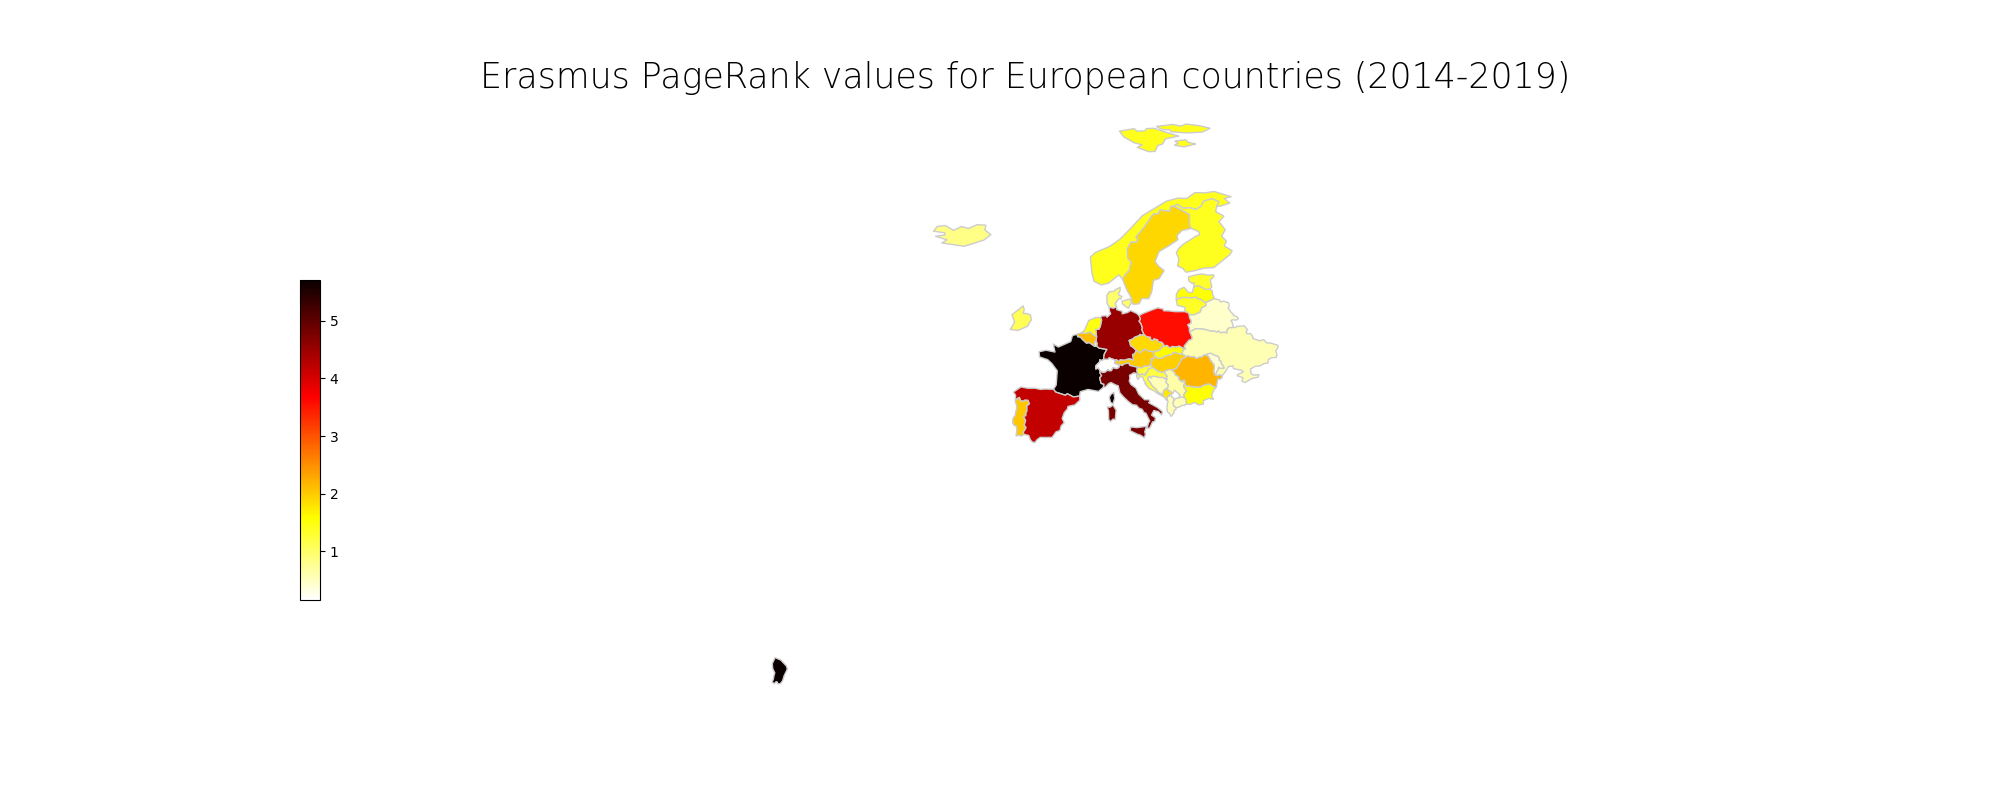
\includegraphics[width=\linewidth]{../geoMaps/PR_geoMap.png}
          \caption{PageRank Heatmap}
         \label{fig:1}
        \end{figure}     

    From the results we obtained it is possible to see that there are some differences between the two methods,
    more in detail in the top results for PageRank and Authorities values there are almost the same countries(France,Italy,Germany,Spain)
     instead the Hubs values are completely different.
    
    \subsection*{Universities Results}
    In the case of the results obtained with the UniNodes graph, we can observe that the PageRank and Hits values 
    have different rankings for top Universities, except for "UNIVERSIDADE DE LISBOA" which is the most important
    for both PageRank and Authorities.
    From the table containing the Hubs scores it is clear that the most relevant Universities in Italy are also the 
    ones that have students traveling to the universities that have high Authorities values. 
    In particular "UNIVERSITA DEGLI STUDI DI ROMA" and "POLITECNICO DI MILANO" have also the top PageRank values.    
    \begin{table}[hbtp]
      \parbox{.25\linewidth}{
        \centering
        \begin{tabular}{l l}
            \hline
            \textbf{Organization} & \textbf{PageRank} \\ \hline
            UNIVERSIDADE DE LISBOA & 49.156703 \\
            Stichting ArtEZ & 45.381767 \\
            UNIVERSITA DEGLI STUDI DI ROMA LA SAPIENZA & 44.403827 \\
            Eesti Kunstiakadeemia & 42.335885 \\
            POLITECNICO DI MILANO & 41.404278\\\hline
          \end{tabular}
          \label{tab:table-label}
        }
      \end{table}

    \begin{table}[hbtp]
        \parbox{.25\linewidth}{
        \centering
        \begin{tabular}{l l}
            \hline
            \textbf{Organization} & \textbf{Authorities} \\ \hline
            UNIVERSIDADE DE LISBOA & 8.715438e+01 \\
            NORGES TEKNISK-NATURVITENSKAPELIGE UNIVERSITET.. & 6.628848e+01 \\
            UNIVERSITAT POLITECNICA DE CATALUNYA & 6.617643e+01 \\
            UNIVERSITAT POLITECNICA DE VALENCIA & 6.022172e+01 \\
            KATHOLIEKE UNIVERSITEIT LEUVEN & 5.544156e+01 \\ \hline
          \end{tabular}
          \label{tab:table-label}
        }
        \end{table}
        \begin{table}[H]
        \parbox{.25\linewidth}{
        \centering
        \begin{tabular}{l l}
            \hline
            \textbf{Organization} & \textbf{Hubs} \\ \hline
            ALMA MATER STUDIORUM - UNIVERSITA DI BOLOGNA & 9.454380e+01 \\
            UNIVERSITA DEGLI STUDI DI PADOVA & 7.960611e+01 \\
            UNIVERSITA DEGLI STUDI DI ROMA LA SAPIENZA & 7.632965e+01 \\
            POLITECNICO DI MILANO & 7.479510e+01 \\
            UNIVERSIDADE DE LISBOA & 6.127300e+01 \\ \hline
          \end{tabular}
          \label{tab:table-label}
        }
        \end{table}
    
    \section{Further analysis and improvements}
    \begin{enumerate}
        \item Use of the \textbf{Random graphs} method to verify if the features we extracted actually give out interesting information;
        \item 
    \end{enumerate} 
    \end{document}